\newpage
\section{Training Stability: depth}\label{appx:depth_experiment}

We report the $\ell_2$-norm of the gradient for each iteration training for models of different stochastic depth in Figure \ref{fig:grad_norm_depth}. We observe very high gradient norms for the first few training iterations but no spikes at later stages of training. 
This happens because we did not initiate the KL-term to be zero at the beginning of the training and it tends to be large at the initialization step for very deep VAEs. 
However, we did not observe our model diverge since the gradient is clipped to reasonable values (200 in these experiments) and after the first few gradient updates, the KL-term goes to reasonable values.
Moreover, we plot training and validation losses in Figure \ref{fig:losses_depth}.

\begin{figure}[!htbp] 
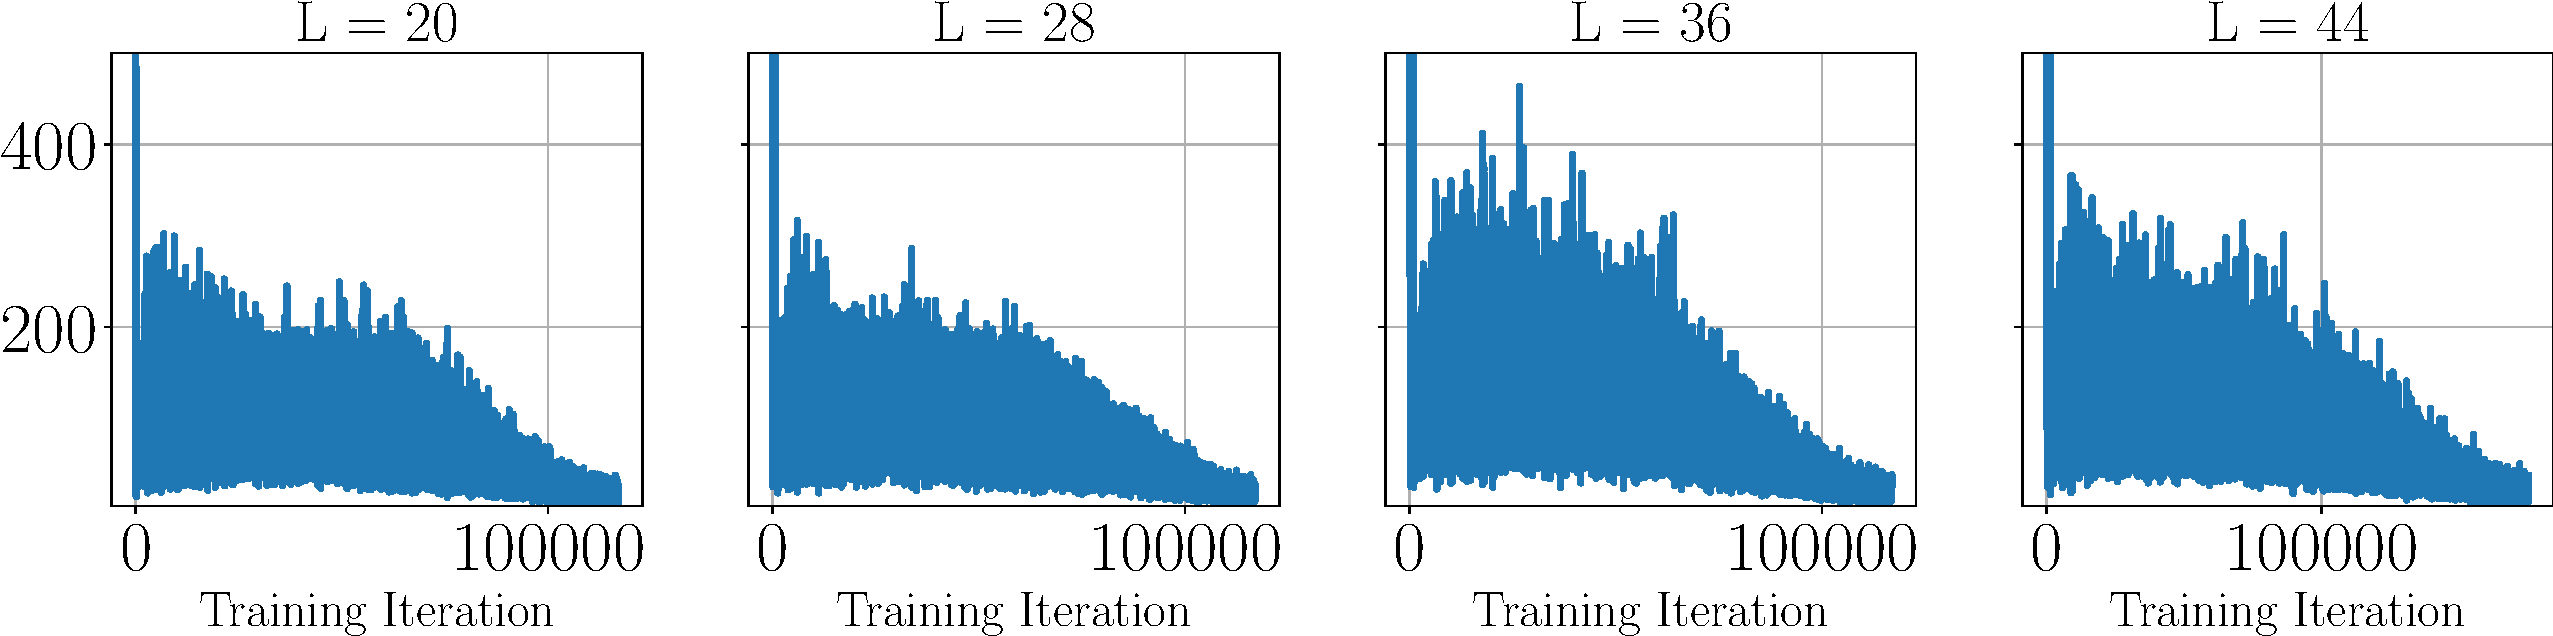
\includegraphics[width=\textwidth]{pics/5_dvp/cifar_depth_grad_norm.pdf}
\caption{The gradient norm at each training iteration. Models were trained on CIFAR10 with different stochastic depths $\mathrm{L}$.}
\label{fig:grad_norm_depth}
\end{figure}

\begin{figure}[!htbp] 
\centering
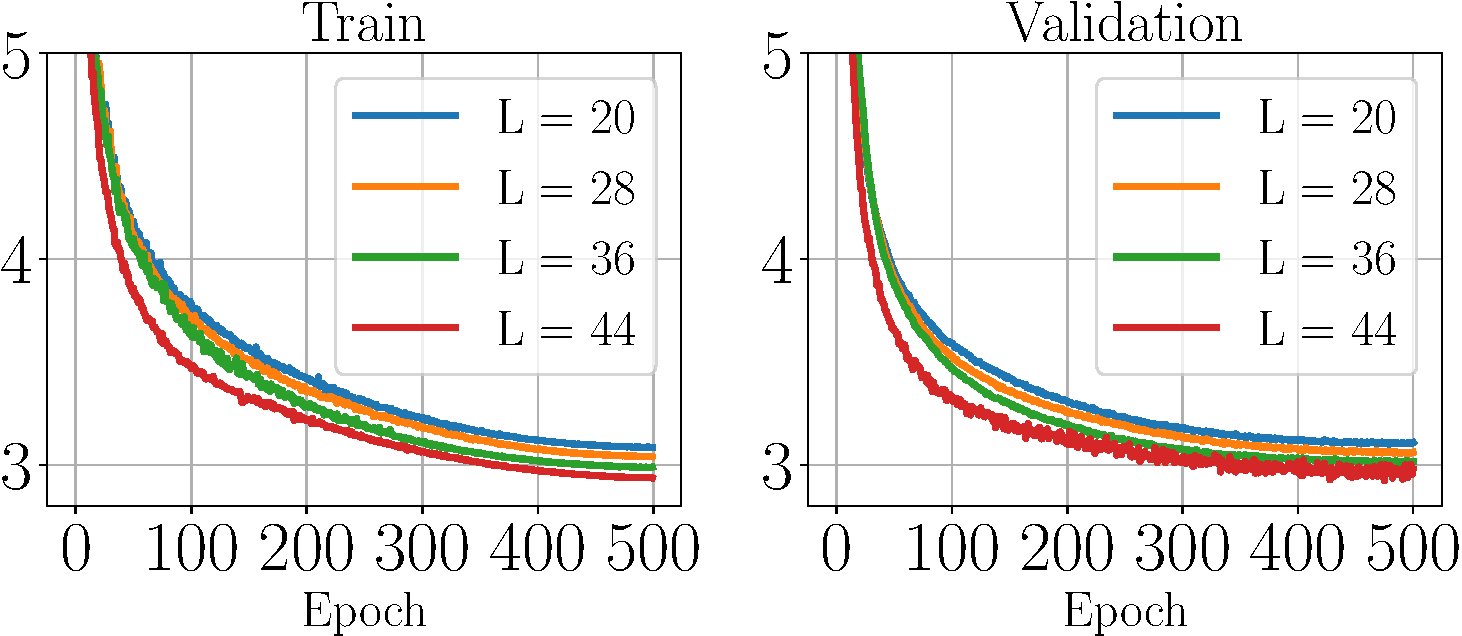
\includegraphics[width=0.7\textwidth]{pics/5_dvp/cifar_depth_losses.pdf}
\caption{The ELBO per pixel on train (left) and validation (right) dataset. Models were trained on CIFAR10 with different stochastic depths $\mathrm{L}$.}
\label{fig:losses_depth}
\end{figure}

\newpage
\section{Model details}

\subsection{Hyperparameters}\label{appendix:hyperparams}
In Table \ref{tab:5_dvp_setup}, we report all hyperparameter values that were used to train the DVP-VAE.

\paragraph{The pseudoinput prior}
We use the diffusion generative model as a prior over pseudoinputs. As a backbone, we use the UNet implementation from \citep{dhariwal2021diffusion}, available on GitHub\footnote{https://github.com/openai/guided-diffusion} with the hyperparameters provided in Table \ref{tab:5_dvp_setup}.

\begin{table}[h]
\caption{Full list of hyperparameters.}
\label{tab:5_dvp_setup}
\begin{center}
% \resizebox{.99\textwidth}{!}{
\begin{tabular}{ll||cc|cc|cc}
\toprule
& &  \multicolumn{2}{c|}{MNIST}   & \multicolumn{2}{c|}{OMNIGLOT} 
% & \multicolumn{2}{c|}{SVHN}   
& \multicolumn{2}{c}{CIFAR10} \\
% & & VAE & DCT-VAE & VAE & DCT-VAE 
% % & VAE & DCT-VAE 
% & VAE & DCT-VAE \\ 
\midrule
\small{\multirow{11}{*}{\STAB{\rotatebox[origin=c]{90}{Optimization}}}} 
& \# Epochs              & \multicolumn{2}{c|}{300}     
                         & \multicolumn{2}{c|}{500}
                         & \multicolumn{2}{c}{3000}
\\
& Batch Size (per GPU)   & \multicolumn{2}{c|}{250}     & \multicolumn{2}{c|}{250}
                         & \multicolumn{2}{c}{128}
\\
& \# GPUs                & \multicolumn{2}{c|}{1}       & \multicolumn{2}{c|}{1}
                         & \multicolumn{2}{c}{1}
\\
& Optimizer              & \multicolumn{2}{c|}{Adamax}  
                         & \multicolumn{2}{c|}{Adamax}  
                         & \multicolumn{2}{c}{Adamax} 
\\
& Scheduler              &  \multicolumn{2}{c|}{Cosine} 
                         & \multicolumn{2}{c|}{Cosine} 
                         & \multicolumn{2}{c}{Cosine}
\\
& Starting LR            &  \multicolumn{2}{c|}{1e-2}   
                         & \multicolumn{2}{c|}{1e-2} 
                         & \multicolumn{2}{c}{3e-3} 
\\ 
& End LR                 &  \multicolumn{2}{c|}{1e-5}   
                         & \multicolumn{2}{c|}{1e-4} 
                         & \multicolumn{2}{c}{1e-4}
\\ 
& LR warmup (epochs)     &  \multicolumn{2}{c|}{2}   
                         & \multicolumn{2}{c|}{2} 
                         & \multicolumn{2}{c}{5}
\\ 
& Weight Decay           &  \multicolumn{2}{c|}{1e-6}   
                         & \multicolumn{2}{c|}{1e-6} 
                         & \multicolumn{2}{c}{1e-6}
\\
& EMA rate               & \multicolumn{2}{c|}{0.999}       & \multicolumn{2}{c|}{0.999}
                         & \multicolumn{2}{c}{0.999}
\\
& Grad. Clipping         & \multicolumn{2}{c|}{5}       
                         & \multicolumn{2}{c|}{2}   
                         & \multicolumn{2}{c}{150}
\\
& $\log\sigma$ clipping  & \multicolumn{2}{c|}{-10}       
                         & \multicolumn{2}{c|}{-10}   
                         & \multicolumn{2}{c}{-10}
\\
\midrule
\multirow{7}{*}{\STAB{\rotatebox[origin=c]{90}{Latents}}} 
& L                             & \multicolumn{2}{c|}{8}              
                                & \multicolumn{2}{c|}{8}         
                                &  \multicolumn{2}{c}{28}
\\
& \multirow{4}{*}{Latent Sizes} & &
                                & &
                                & \multicolumn{2}{c}{$10\times32^2$,}
\\
&                               & \multicolumn{2}{c|}{$4\times14^2$,}  
                                & \multicolumn{2}{c|}{$4\times14^2$,}
                                & \multicolumn{2}{c}{$8\times16^2$.}
\\
&                               & \multicolumn{2}{c|}{$4\times7^2$.}  
                                & \multicolumn{2}{c|}{$4\times7^2$.}
                                & \multicolumn{2}{c}{$6\times8^2$,}
\\
&                               & &
                                & &
                                & \multicolumn{2}{c}{$4\times4^2$.}
\\
& Latent Width (channels)       & \multicolumn{2}{c|}{1}             
                                & \multicolumn{2}{c|}{1}          
                                & \multicolumn{2}{c}{3} 
\\
& Context Size                  & \multicolumn{2}{c|}{$1\times7\times7$ } 
                                & \multicolumn{2}{c|}{$1\times5\times5$ }    
                                & \multicolumn{2}{c}{$3\times7\times7$ }
\\ \midrule
\multirow{6}{*}{\STAB{\rotatebox[origin=c]{90}{Architecture}}} 
& $N_{\text{enc}}$ blocks       &  \multicolumn{2}{c|}{3}            
                                &  \multicolumn{2}{c|}{3} 
                                &  \multicolumn{2}{c}{4} 
\\
& ResBlock  $C_{in}$              &  \multicolumn{2}{c|}{32}            
                                &  \multicolumn{2}{c|}{80} 
                                &  \multicolumn{2}{c}{128} 
\\
& ResBlock  $C_{hid}$             &  \multicolumn{2}{c|}{32}            
                                & \multicolumn{2}{c|}{40}
                                &  \multicolumn{2}{c}{96} 
\\
& Activation                    & \multicolumn{2}{c|}{SiLU}  
                                & \multicolumn{2}{c|}{SiLU}
                                & \multicolumn{2}{c}{SiLU}
\\
& Likelihood                    & \multicolumn{2}{c|}{Bernoulli}  
                                & \multicolumn{2}{c|}{Bernoulli}
                                & \multicolumn{2}{c}{Discretized Logisitc}
\\
& \# mixture comp                & \multicolumn{2}{c|}{---}  
                                & \multicolumn{2}{c|}{---}
                                & \multicolumn{2}{c}{10}
\\
\midrule
\small{\multirow{7}{*}{\STAB{\rotatebox[origin=c]{90}{Context Prior}}}} 
& \# Diffusion Steps     & \multicolumn{2}{c|}{50}  
                         & \multicolumn{2}{c|}{50}
                         & \multicolumn{2}{c}{50}
\\
& \# Scales in UNet      & \multicolumn{2}{c|}{1}  
                         & \multicolumn{2}{c|}{1}
                         & \multicolumn{2}{c}{1}
\\
& \# ResBlocks per Scale & \multicolumn{2}{c|}{2}  
                         & \multicolumn{2}{c|}{2}
                         & \multicolumn{2}{c}{3}
\\
& \# Channels            & \multicolumn{2}{c|}{16}  
                         & \multicolumn{2}{c|}{16}
                         & \multicolumn{2}{c}{32}
\\
& $\beta$ schedule       & \multicolumn{2}{c|}{linear}  
                         & \multicolumn{2}{c|}{linear}
                         & \multicolumn{2}{c}{linear}
\\
& $\log$ SNR min         & \multicolumn{2}{c|}{-6}  
                         & \multicolumn{2}{c|}{-6}
                         & \multicolumn{2}{c}{-10}
\\
& $\log$ SNR max         & \multicolumn{2}{c|}{7}  
                         & \multicolumn{2}{c|}{7}
                         & \multicolumn{2}{c}{7}
\\
\bottomrule
\end{tabular}
\end{center}
\end{table}


\newpage
\section{Samples}\label{appendix:samples}

In Figure \ref{fig:all_samples}, we present non-cherry-picked unconditional samples from our DVP-VAE and in Figure~\ref{fig:ctx_samples} we present non-cherry-picked unconditional samples from the pseudoinput prior $\hat{r}(\rvu)$.

\begin{figure}[!htbp]
    \centering
    \begin{tabular}{ccc}
    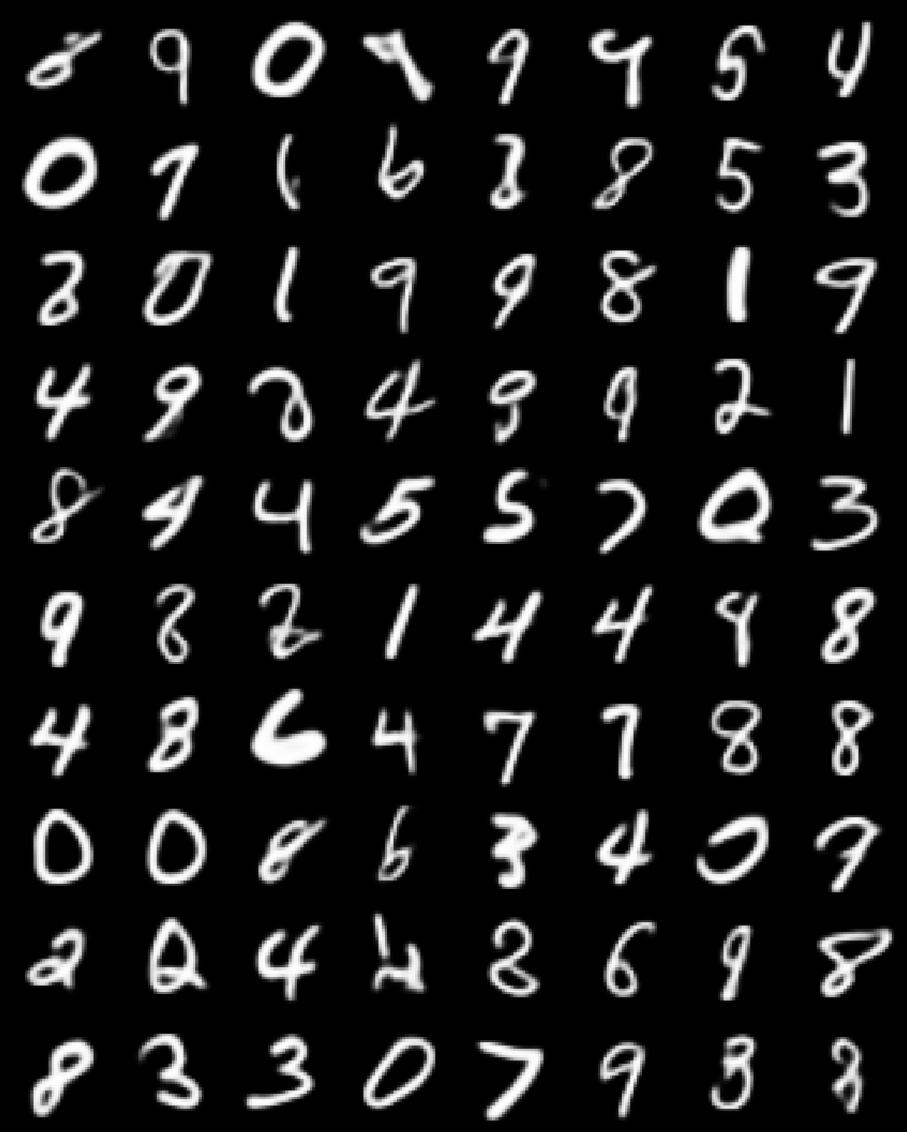
\includegraphics[width=0.3\textwidth]{pics/5_dvp/mnist_samples_t0.7.pdf} &  
        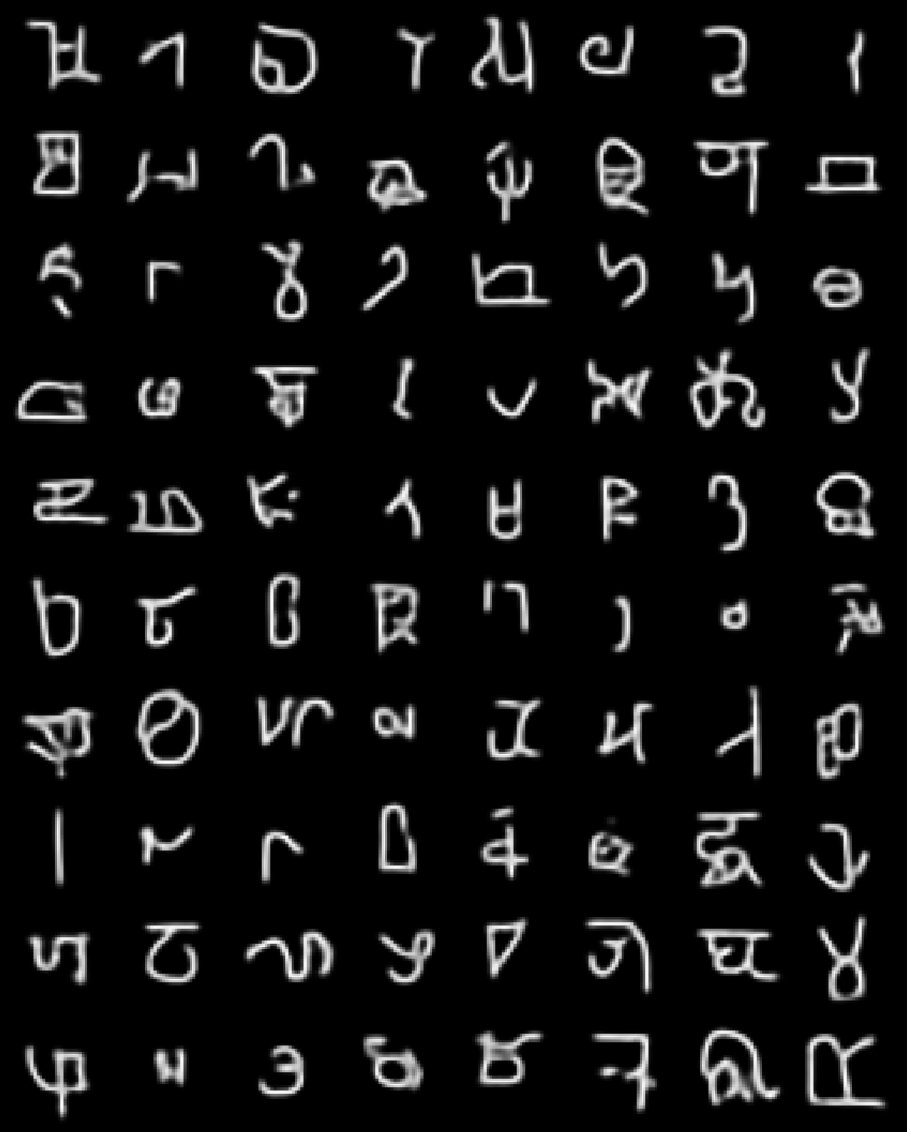
\includegraphics[width=0.3\textwidth]{pics/5_dvp/omniglot_samples_t0.7.pdf} & 
        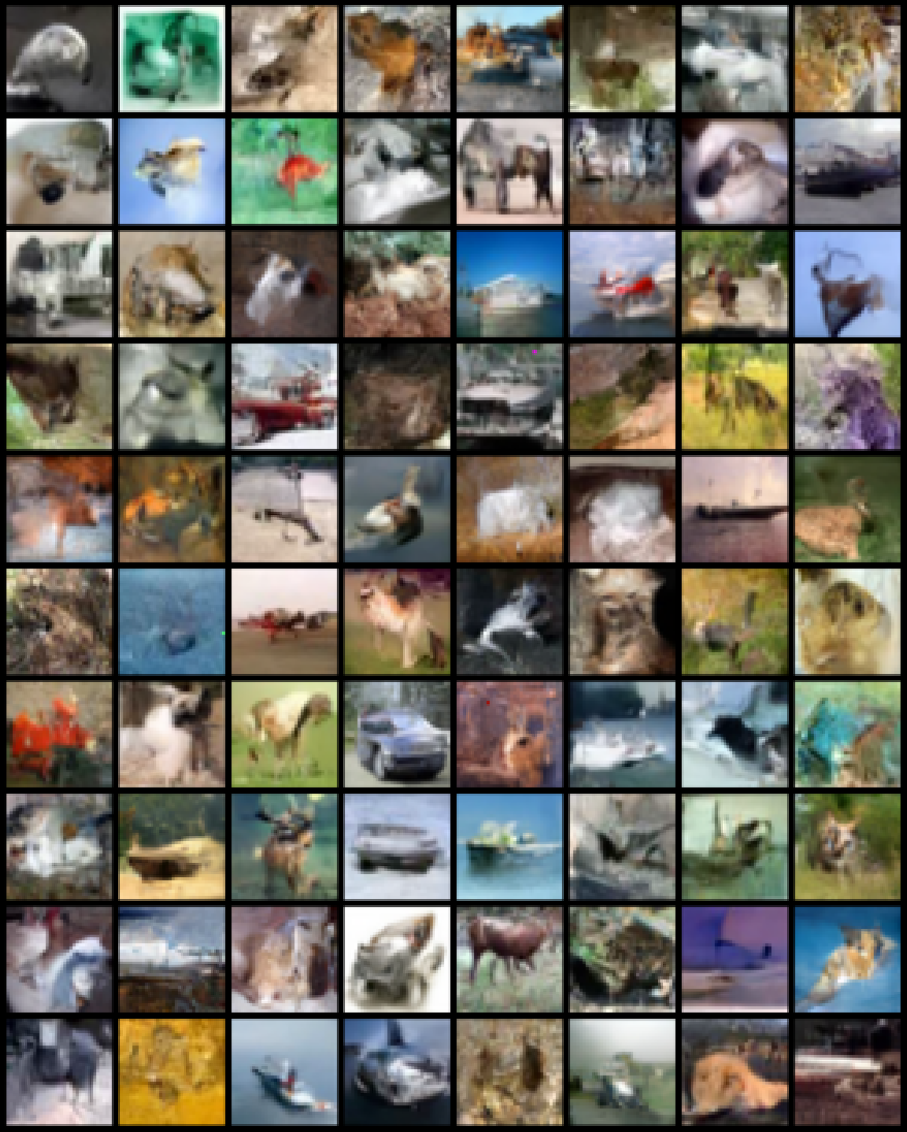
\includegraphics[width=0.3\textwidth]{pics/5_dvp/cifar10_samples_t0.7.pdf}\\
        (a) MNIST  & (b) OMNIGLOT & (c) Cifar10\\
        % \includegraphics[width=0.75\textwidth]{pics/mnist_dct_vae_sample.pdf} \\
        % (a) DCT-VAE \\
    \end{tabular}
    \caption{Uncoditional samples.}
    \vskip -10pt
    \label{fig:all_samples}
\end{figure}

\begin{figure}[!htbp]
    \centering
    \begin{tabular}{ccc}
    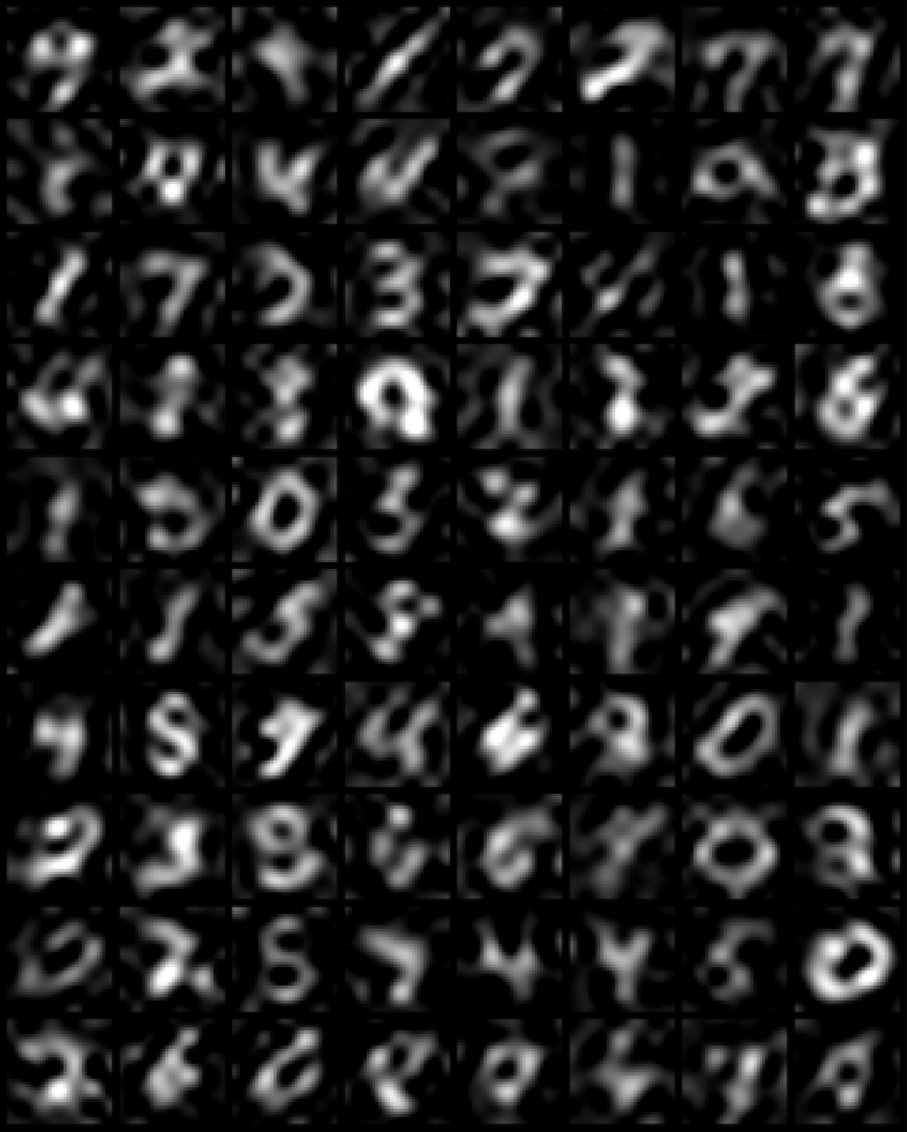
\includegraphics[width=0.3\textwidth]{pics/5_dvp/mnist_ctx_samples.pdf} &  
        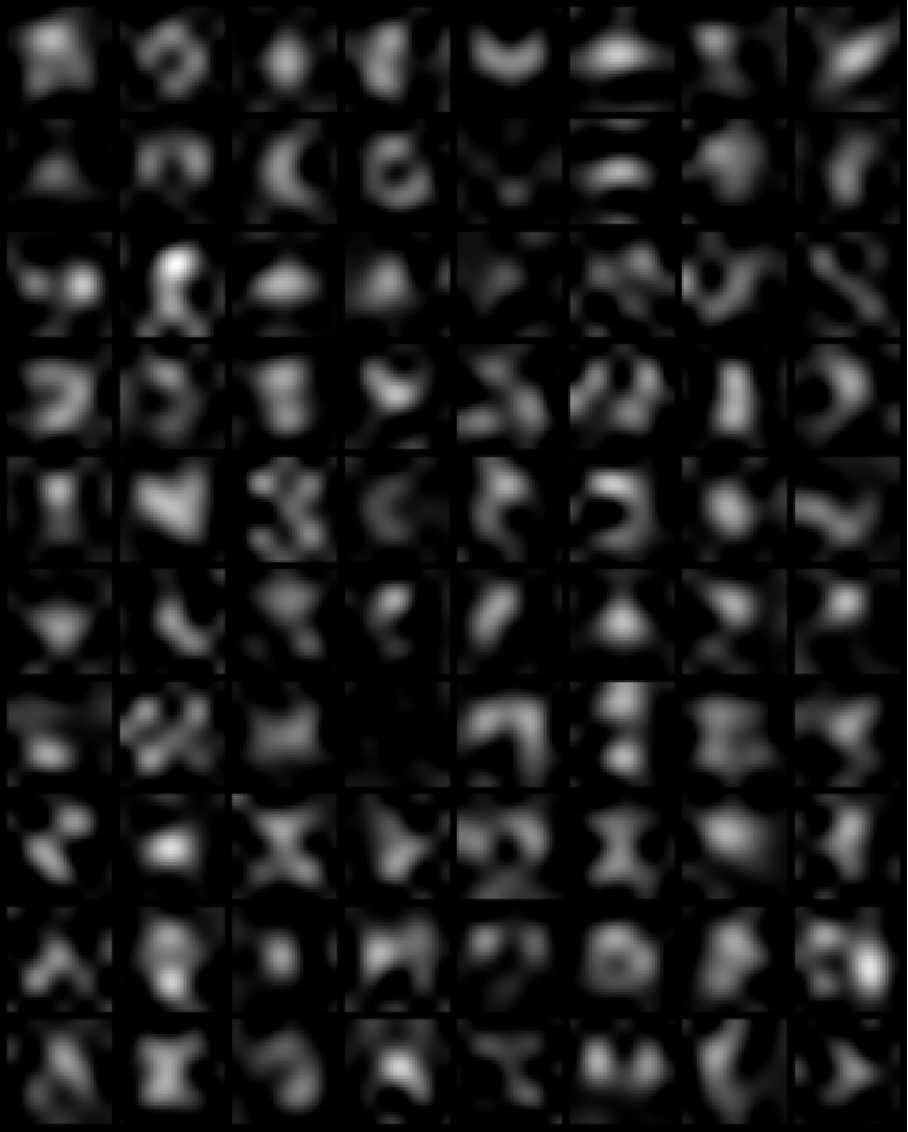
\includegraphics[width=0.3\textwidth]{pics/5_dvp/omniglot_ctx_samples.pdf} & 
        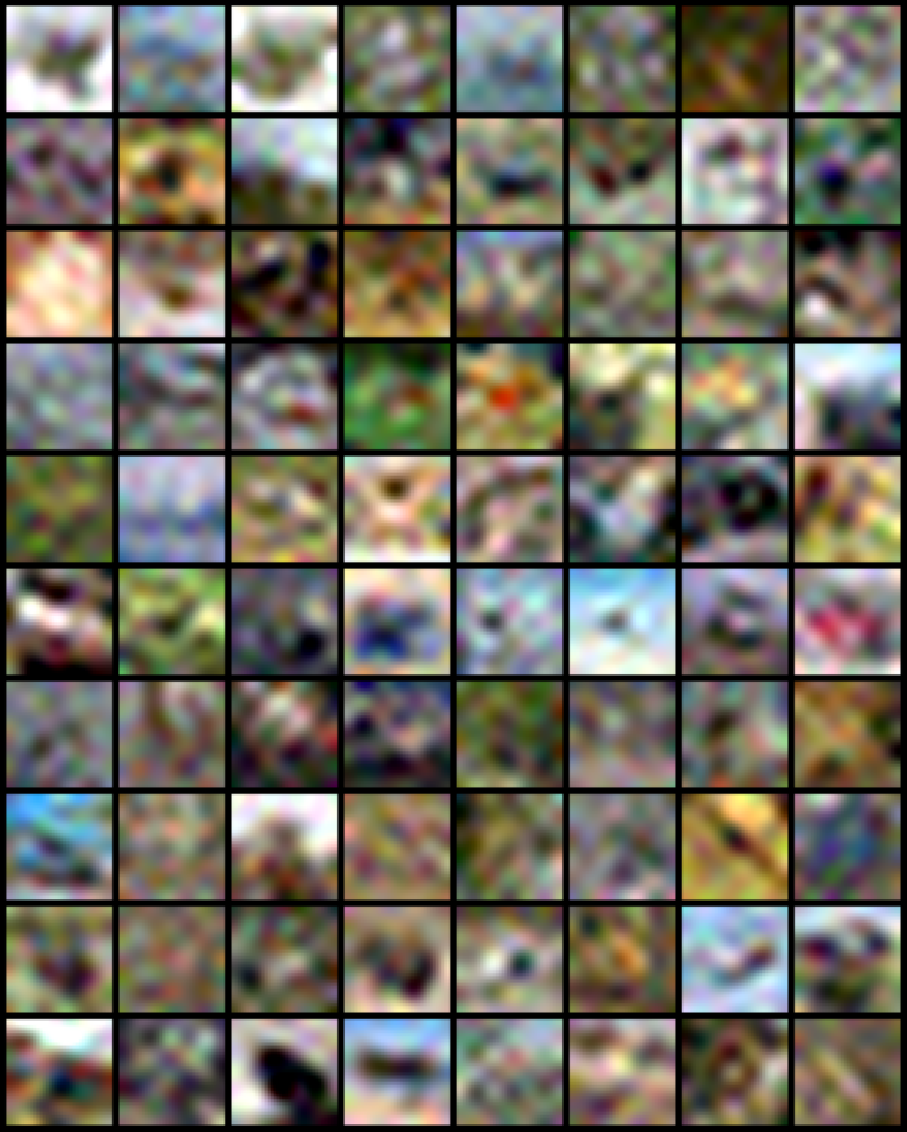
\includegraphics[width=0.3\textwidth]{pics/5_dvp/cifar10_ctx_samples.pdf}\\
        (a) MNIST  & (b) OMNIGLOT & (c) Cifar10\\
    \end{tabular}
    \caption{Uncoditional samples of pseudoinputs.}
    \vskip -10pt
    \label{fig:ctx_samples}
\end{figure}


